\subsection{Описание программной разработки}
\label{section:practice}

Разработанное решение реализовано в формате модуля языка Python. Структура модуля изображена на рисунке~\ref{fig:tree}, служебные файлы (такие как \texttt{\_\_init\_\_.py}) опущены.

\begin{figure}
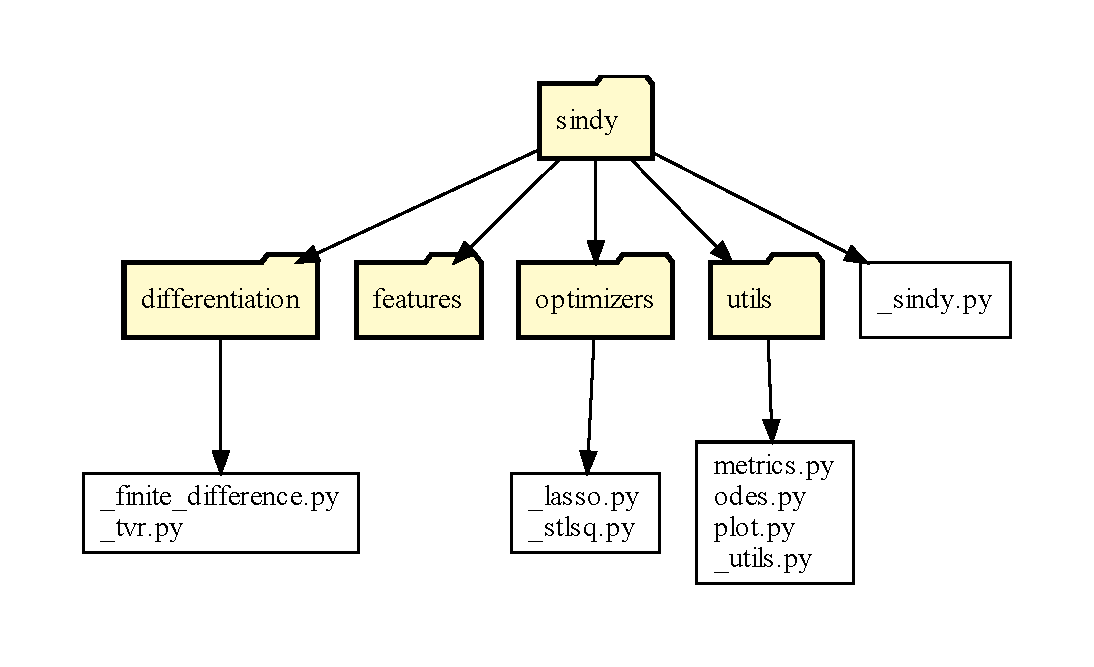
\includegraphics[width=0.85\textwidth]{tree}
\caption{Структура модуля}
\label{fig:tree}
\end{figure}

Для удобства разработки, основные части алгоритма реализованы в отдельных подмодулях.

Подмодуль \texttt{optimizers} содержит реализацию алгоритмов разреженной регрессии. В качестве Lasso используется \texttt{sklearn.linear\_model.Lasso} с зафиксированным параметром \texttt{fit\_intercept=False}, который убирает свободный член из формулы регрессии (считаем, что он задается в матрице признаков, если необходим). STLSQ реализован как \texttt{sklearn.base.RegressorMixin}.

Подмодуль \texttt{differentiation} содержит алгоритмы численного дифференцирования, \texttt{\_finite\_difference.py} --- метод конечных разностей, \texttt{\_tvr.py} --- методы регуляризации полной вариации. Первый метод назван \texttt{FastTVR}, так как не является итеративным и содержит только одну процедуру решения СЛАУ, второй метод --- просто \texttt{TVR}. При описании результатов в подразделе~\ref{section:results} методы указаны именно с этими именами. Все алгоритмы дифференцирования реализованы как \texttt{sklearn.base.TransformerMixin}, методы регуляризации полной вариации используют матрицы дискретных операторов в явном виде.

Подмодуль \texttt{features} не содержит никаких реализаций, поскольку в работе в итоге исследовались только системы с полиномиальными правыми частями, и для получения матрицы признаков использовался \texttt{sklearn.preprocessing.PolynomialFeatures}.

Подмодуль \texttt{utils} содержит различные вспомогательные классы и функции. В частности метрики, используемые системы ОДУ, функции для генерации и визуализации данных.

Алгоритм идентификации реализован в \texttt{\_sindy.py} как \texttt{sklearn.base.BaseEstimator}. \enquote{Обученный} алгоритм может предсказывать значения левых частей системы, а также описать саму систему или составить экземпляр класса \texttt{sindy.utils.Equation}, который затем можно эволюционировать для получения траектории.

Исходный код программной разработки доступен в репозитории по ссылке в приложении А.